\documentclass{article}

\usepackage[utf8]{inputenc}
\usepackage[danish]{babel}
\usepackage{graphicx}

\title{Verbatim, figurer og referencer}
\author{Jon Sporring}
\date{\today}

\begin{document}
\maketitle

\section{Verbatim}
Hvis man vil vise et stykke tekst uden at \LaTeX\ fortolker det som en
række kommandoer, skal man bruge verbatim:
\begin{verbatim}
let rec factorial n =
  if n = 0 then
    1
  else
    n * factorial (n -1)
\end{verbatim}
I verbatim mode skrives alt bogstaveligt.

\section{Matematik}
\LaTeX\ er særlig god til matematik. Man kan både skrive det "`inline"'
som her: $\exp\frac{-x^2}{2}$ eller på en linje for sig:
\begin{equation}
  \label{eq:minLigning}
  f(x) = \exp\left(\frac{-x^2}{2}\right)
\end{equation}
Hvis man har givet ligningen et nummer, så kan man referere til den,
f.eks. (\ref{eq:minLigning}).

\section{Figurer}
Figurer og tabeller kan med fordel skrives i "`floats"', dvs. som
tekstområder, som \LaTeX\ gerne må flytte lidt rundt på. Man kan så
henvise til disse "`floats"' med label-reference systemet, se
f.eks. Figur~\ref{fig:minFigur}.
\begin{figure}
  \centering
  \fbox{Figurens indhold}
  \caption{Dette er underteksten til en figur.}
  \label{fig:minFigur}
\end{figure}
Et eksempel på en table er givet i Tabel~\ref{tab:minTabel}.
\begin{table}
  \centering
  \begin{tabular}{|l|l|l|}
    \hline
    & Blond & Rødhåret \\
    \hline
    Mand & 10 & 14\\
    Kvinde & 23 & 2 \\
    \hline
  \end{tabular}
  \caption{Dette er underteksten til en tabel}
  \label{tab:minTabel}
\end{table}
Vi kan også komme billeder i "`floats"' som vist i Figur~\ref{fig:billede}.
\begin{figure}
  \centering
  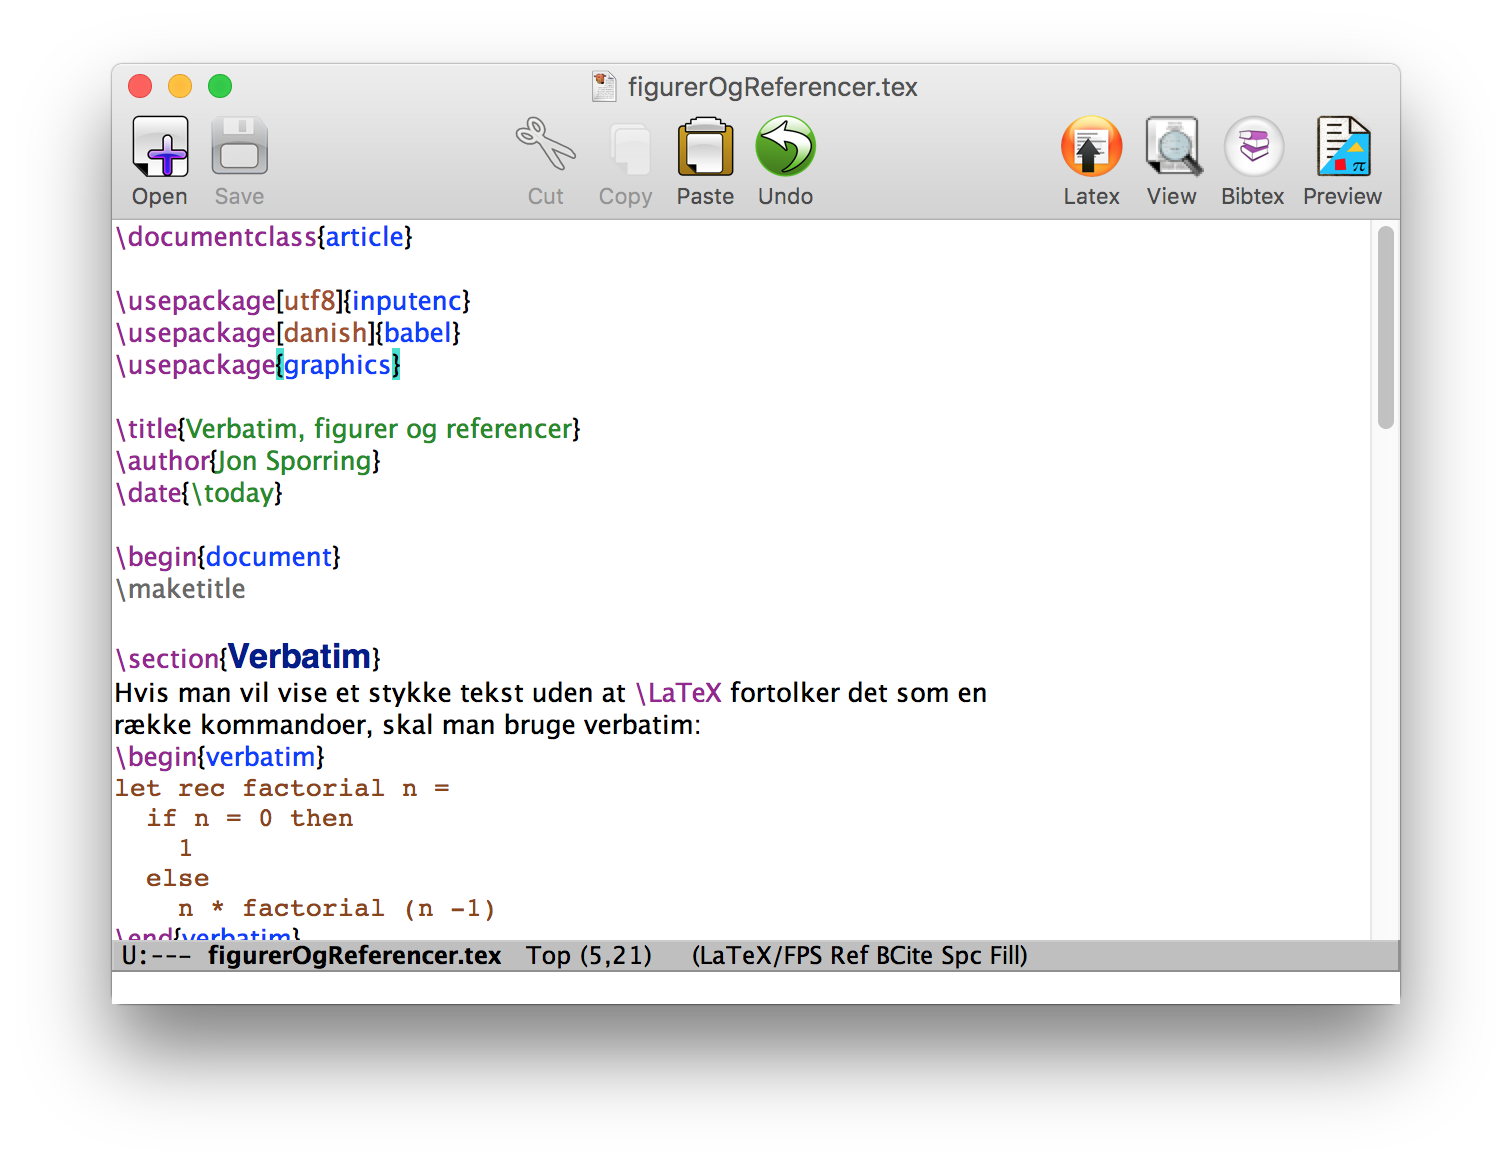
\includegraphics[width=0.6\linewidth]{emacs.png}
  \caption{Dette er et billede i en figur.}
  \label{fig:billede}
\end{figure}
\end{document}
